\section{Desarrollo/Análisis}

Inicialmente se hizo la prueba del giroscopio para determinar que los 3 ejes funcionaran correctamente a la hora de mover la placa.
\begin{figure}[H]
\centering
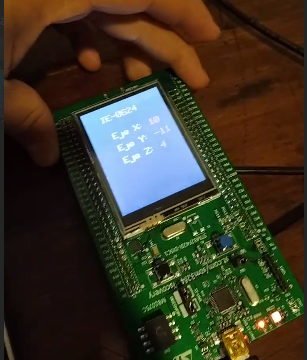
\includegraphics[width=.55\linewidth]{Imagenes/5.png}
 \caption{Funcionamiento del giroscopio.}
 \label{fig_gyro}
\end{figure}
Lo anterior se logró gracias los ejemplos dados de la biblioteca libopencm3. Y realizando otro tipo de depuraciones para darle un estilo a la presentación en la pantalla LCD.\par
Lo siguiente que se hizo fue la configuración de los GPIO's y establecer el pin \texttt{PA0} como entrada analógico y poder mostrar la tensión que posee la batería en el momento que es conectada. Inicialmente se hizo un divisor de tensión a partir de $v_{in}=\SI{9}{\volt}$, junto con resistencias de \SI{1.8}{\kilo\ohm} y \SI{1}{\kilo\ohm}, obtiendo una tensión de \SI{3.2}{\volt} tal como se muestra a continuación.
\begin{figure}[H]
\centering
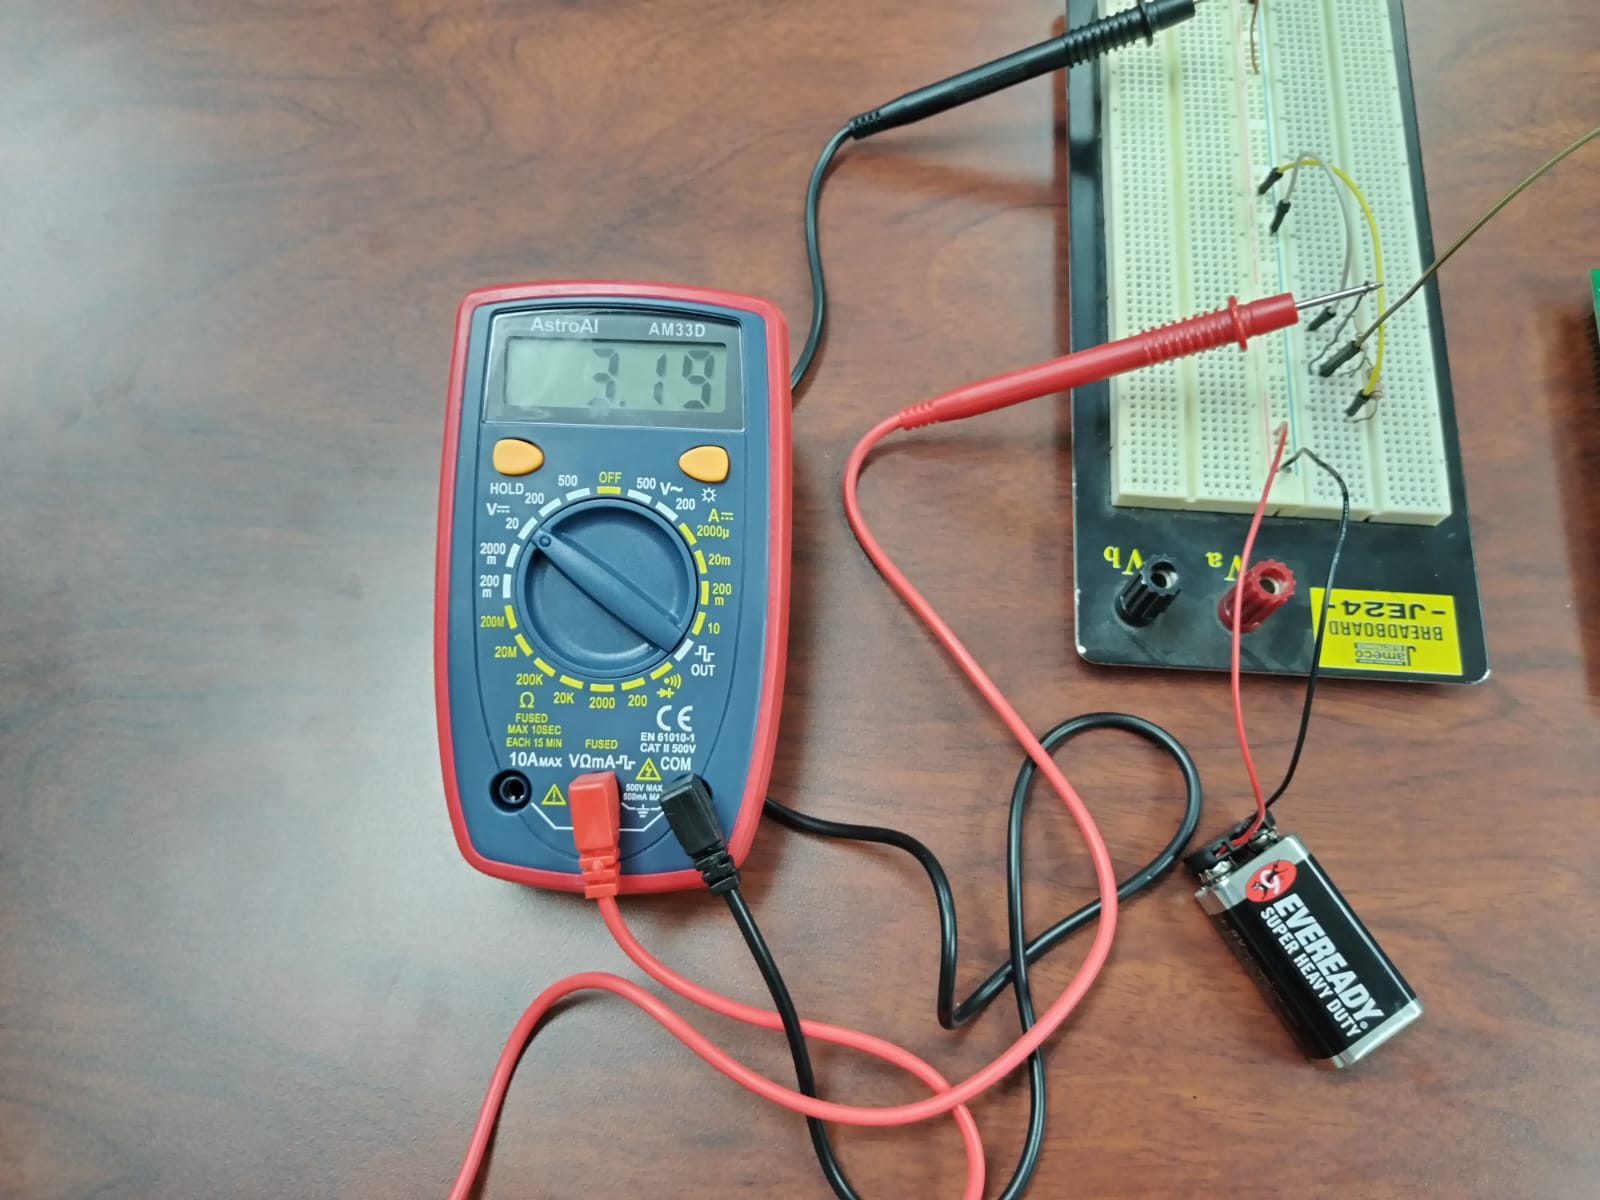
\includegraphics[width=.55\linewidth]{Imagenes/6.jpeg}
 \caption{Tensión de salida}
 \label{fig_vout}
\end{figure}
Esta tensión eléctrica es la que recibirá la placa por medio del pin \texttt{PA0}.
\begin{figure}[H]
\centering
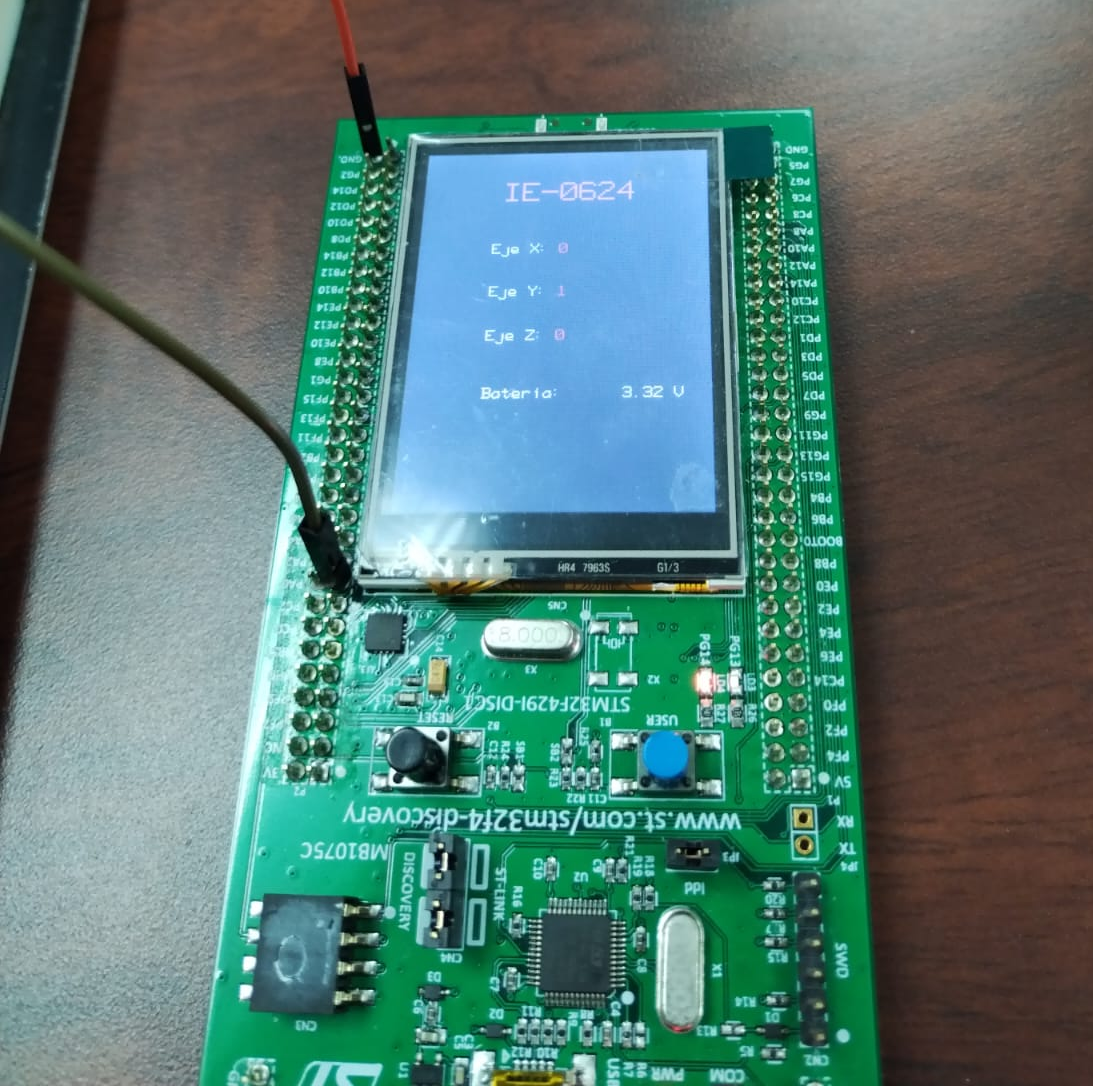
\includegraphics[width=.55\linewidth]{Imagenes/7.png}
 \caption{Magnitud de la batería menor a \SI{7}{\volt}.}
 \label{fig_bat}
\end{figure}
Además, note que de la figura anterior se muestra un LED encendido, lo cual indica una alarma ya que su valor es menor de \SI{7}{\volt}, sino fuera así, entonces el LED no debe encenderse.
\begin{figure}[H]
\centering
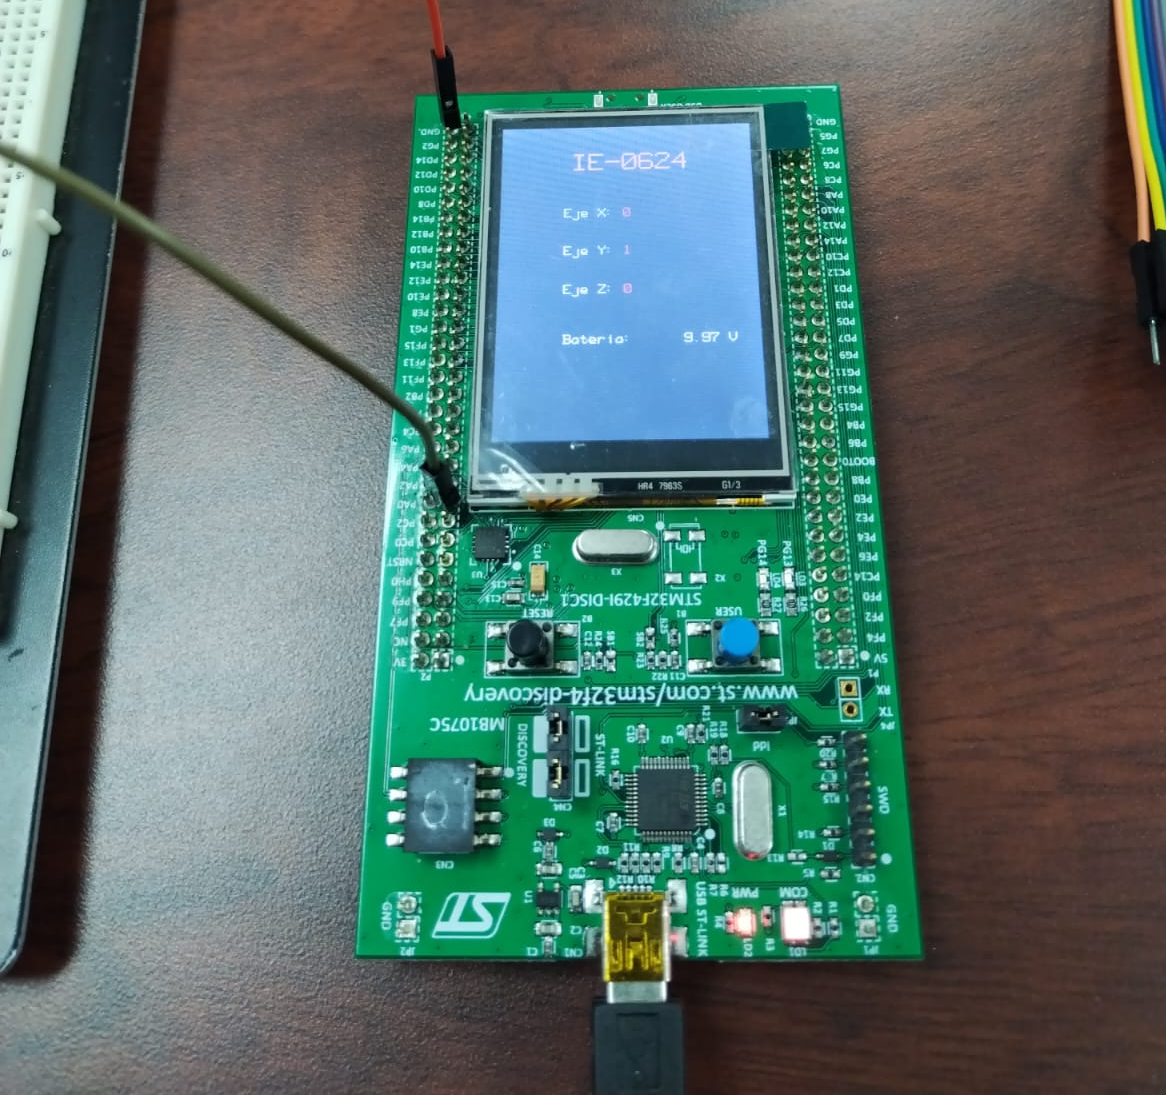
\includegraphics[width=.55\linewidth]{Imagenes/8.png}
 \caption{Magnitud de la batería mayor a \SI{7}{\volt}.}
 \label{fig_bat_OFF}
\end{figure}
Note que el LED \texttt{PG14} no se enciende, lo cual esta correctamente realizado.

\newpage